\chapter{Methods and materials}
\label{cap:metodologia}

Chapter~\ref{cap:contexto} established that the three questions of the retail investor have an
answer in the literature but not in any free tool. This chapter describes the options taken to
answer them. It first presents the research methodology and the datasets. It then describes the
four methods selected, one for each decision the system has to take. It indicates the tools
employed. And it finally states the technological and social challenges of the domain.

\section{Research methodology}
\label{sec:met_metodologia}

This dissertation is framed within design science research \autocite{hevner2004design}, in which
the object of study is an artefact built to solve a class of problem and the knowledge produced
resides both in the artefact and in the process of its evaluation. It is the appropriate framing
when the contribution is a system, and it differs from a purely empirical study in that the object
evaluated does not exist before it is built.

The design science literature establishes that the evaluation of the artefact must be rigorous and
constitute a central activity of the process, and not a final confirmation step
\autocite{hevner2004design, peffers2007dsrm}. This requirement is met through three commitments
made before the experiments were carried out.

The first consists in comparing each component with a simpler alternative, selected and declared
before the measurement is carried out, so that the result can be negative. The second consists in
fixing the success criterion of each comparison together with the metric, and not after observing
the values obtained. The third consists in evaluating the artefact twice: over held-out historical
data and, subsequently, in operation, over the decisions the system takes autonomously in
production. The third evaluation is the least common of the three and is the one that produces the
result described in Section~\ref{sec:av_producao}.

The requirement is not met in full, and the gap is declared. Utility, in the sense in which the
design science literature employs the term, is utility for whoever uses the artefact, and that
property is determined with users. What this dissertation measured is the faithfulness of the
explanations produced, a property that belongs to the system; utility, which depends on the
relation between the system and whoever reads it, remains unmeasured.

The system takes four distinct decisions, shown in Figure~\ref{fig:met_decisoes}. The first three
correspond to the three investor questions stated in Chapter~\ref{cap:introducao}; the fourth is
not a question of the investor, but of the system itself, and exists because answering the first
three does not imply interrupting the user.

\begin{figure}[ht]
\centering
\begin{tikzpicture}[
  font=\small, >={Stealth[length=2.4mm]},
  cx/.style={draw, rounded corners, align=center, text width=2.85cm, minimum height=2.0cm,
             inner sep=4pt, fill=black!4},
  num/.style={font=\bfseries\small, text=black!45},
]
  \node[cx] (a) {\textbf{1. Is it unusual?}\\[3pt]
    \footnotesize compare today with\\ \footnotesize normal for \emph{this} company};
  \node[cx, right=0.6cm of a] (b) {\textbf{2. Company or}\\\textbf{market?}\\[3pt]
    \footnotesize split the movement\\ \footnotesize into its sources};
  \node[cx, right=0.6cm of b] (c) {\textbf{3. Has it happened before?}\\[3pt]
    \footnotesize retrieve past cases\\ \footnotesize and measure what followed};
  \node[cx, right=0.6cm of c] (d) {\textbf{4. Worth alerting?}\\[3pt]
    \footnotesize decide whether this warrants\\ \footnotesize interrupting someone};
  \node[num, above=1mm of a] {statistics};
  \node[num, above=1mm of b] {regression};
  \node[num, above=1mm of c] {meaning};
  \node[num, above=1mm of d] {learning};
  \draw[->, thick, black!50] (a) -- (b);
  \draw[->, thick, black!50] (b) -- (c);
  \draw[->, thick, black!50] (c) -- (d);
\end{tikzpicture}
\caption[The four decisions of the system]{The four decisions of the system and the family of
techniques associated with each. The first three correspond to the questions stated in
Chapter~\ref{cap:introducao}. Each column corresponds to a section of this chapter, between
Section~\ref{sec:met_detecao} and Section~\ref{sec:met_triagem}.}
\label{fig:met_decisoes}
\end{figure}


\section{Datasets}
\label{sec:met_dados}

This section describes the datasets used in the training and evaluation of the system, as well as
the records produced by the system in operation.

The historical layer rests on \gls{FNSPID} \autocite{dong2024fnspid}, a public corpus of financial
news that associates a date and a company with each headline. The corpus contains no prices, no
market reaction and no indication of relevance: that information is built in this work, by aligning
each headline with the corresponding price series. From the alignment comes the training set of the
triage model, with 79{,}753 examples.

The evaluation of the anomaly detector uses a distinct dataset, made up of three years of daily
quotes. The choice of a separate set is deliberate: the evaluation requires variety of volatility
across companies, whereas the list monitored in production is a product decision. Evaluating the
detector on exactly the set it was built to serve would produce a measurement with no informative
value.

All prices used are closes adjusted for splits and dividend distributions. The adjustment is not a
detail in the period considered, which contains a four-for-one split of Apple and two of Tesla: on
unadjusted series, the detector would flag falls of thirty to eighty per cent on days with no event
at all.

Table~\ref{tab:met_conjuntos} brings together the datasets used, and
Table~\ref{tab:met_universos} the company sets, whose counts differ for reasons described in the
respective column.

\begin{table}[!htbp]
\caption[Datasets used]{Datasets used in the work, with the time span and the size read from the
files. The last three rows correspond to the system in operation.}
\label{tab:met_conjuntos}
\centering
\small
\begin{tabular}{L{0.30\textwidth} L{0.26\textwidth} L{0.34\textwidth}}
\toprule
\tabhead{Dataset} & \tabhead{Span} & \tabhead{Size} \\
\midrule
\multicolumn{3}{l}{\emph{Historical}} \\
Triage training set & 2018-01-02 to 2023-12-18 & $79{,}753$ examples, 14 companies \\
Prices for the detection evaluation & 2023-06-01 to 2026-06-01 & 15 companies, $\approx 750$ days each \\
\midrule
\multicolumn{3}{l}{\emph{Operation}} \\
Reconstructed precedent base & one year of own collection & $38{,}214$ cases with measured impact \\
Alerts delivered & 2026-07-09 to 2026-08-13 & 367 messages \\
Triage decision log & 2026-07-22 to 2026-08-20 & $36{,}925$ decisions \\
\bottomrule
\end{tabular}
\end{table}

\begin{table}[!htbp]
\caption[Company sets]{Company sets used. The counts differ because each set serves a distinct
purpose. The sets are not nested: the list monitored in production contains two companies absent
from every historical set and a third that appears in the canonical map but not in the triage
dataset.}
\label{tab:met_universos}
\centering
\small
\begin{tabular}{L{0.30\textwidth} C{0.10\textwidth} L{0.48\textwidth}}
\toprule
\tabhead{Set} & \tabhead{Companies} & \tabhead{Purpose} \\
\midrule
Extended sector map & 17 & Universe covered by the movement decomposition \\
Canonical historical map & 15 & Relevance label in the retrieval evaluation \\
Prices for detection & 15 & Variety of volatility in the detector evaluation \\
Triage dataset & 14 & Result of the alignment between news and prices \\
\quad covered by the training block & 13 & Companies actually present in training \\
\quad covered by the test block & 9 & Companies present in the evaluation \\
List monitored in production & 12 & Product decision \\
\bottomrule
\end{tabular}
\end{table}

\section{Detection of unusual movements}
\label{sec:met_detecao}

The first decision of the system consists in determining whether the movement observed on a day is
unusual for the company in question. A fixed threshold rule, of the kind that flags changes above
three per cent, is inadequate for this purpose, because the same percentage corresponds to events
of very different rarity depending on the volatility of the company.

The method adopted belongs to the statistical family of the anomaly detection taxonomy
\autocite{chandola2009anomaly}, which defines normality from the recent distribution of the data
themselves. The movement of the day is compared with the recent behaviour of the same stock and
expressed in standard deviations:

\begin{equation}
z_t = \frac{r_t - \mu}{\sigma}
\label{eq:zscore}
\end{equation}

where $r_t$ is the logarithmic return of the day, $r_t = \ln(P_t / P_{t-1})$, and $\mu$ and
$\sigma$ are the mean and the standard deviation of the returns of the twenty preceding days. The
use of logarithmic returns follows the current convention in financial series, since it makes
returns additive over time and symmetric between rises and falls. The values presented therefore
differ from those displayed by a stock application: a logarithmic return of $+19.82\%$ corresponds
to a price change of $+21.92\%$.

The window slides each day, and the day being assessed is excluded from the window that defines
its own norm, as shown in Figure~\ref{fig:met_janela}. Without this exclusion, the day would
contribute to the mean and to the standard deviation against which it is compared, attenuating its
own anomaly. The same discipline prevents the use of any information posterior to the day being
assessed.

\begin{figure}[ht]
\centering
\begin{tikzpicture}[font=\small, >={Stealth[length=2.2mm]}]
  % barras dos dias
  \foreach \i in {0,...,19} {
    \fill[black!18] (\i*0.32,0) rectangle (\i*0.32+0.24,0.55);
  }
  \fill[orange!70] (20*0.32,0) rectangle (20*0.32+0.24,1.25);
  \draw[decorate, decoration={brace, amplitude=5pt}, black!55]
    (0,-0.15) -- (19*0.32+0.24,-0.15)
    node[midway, below=6pt, align=center, black!65]
    {\footnotesize the \textbf{20 preceding days}\\[-2pt]\footnotesize give $\mu$ and $\sigma$};
  \draw[decorate, decoration={brace, amplitude=5pt}, orange!75!black]
    (20*0.32,-0.15) -- (20*0.32+0.24,-0.15)
    node[midway, below=6pt, align=center, text=orange!60!black]
    {\footnotesize the day\\[-2pt]\footnotesize \textbf{being judged}};
  \draw[->, thick, black!45] (20*0.32+0.6,0.6) -- (20*0.32+1.5,0.6)
    node[right, align=left, black!60] {\footnotesize tomorrow the window\\[-2pt]\footnotesize slides one day};
\end{tikzpicture}
\caption[The rolling window of the \emph{z}-score]{The window that establishes the usual behaviour
of the stock. The day being assessed is \textbf{left out} of the computation of the norm against
which it is compared, a separation that prevents the use of information unavailable at the moment
of the decision.}
\label{fig:met_janela}
\end{figure}

The separation is not merely a convention of writing: it is a slice.
Listing~\ref{lst:janela} reproduces the calculation as it is executed. The line that
guarantees it is the fifth, in which the interval ends at the penultimate element and
excludes, by construction, the day being assessed.

\begin{lstlisting}[caption={[The window that excludes the day assessed]The window that
excludes the day assessed. The interval \texttt{[-window-1:-1]} ends before the last element,
so the return of the day under assessment does not enter the mean or the standard deviation
against which it is compared. The body of the detection function is reproduced, without the
indentation it carries in the source file. The comment is in the original.}, label={lst:janela}]
r = pd.Series(list(returns), dtype="float64").dropna().reset_index(drop=True)
if len(r) < window + 1:
    raise ValueError(f"São precisos pelo menos {window + 1} retornos (recebidos {len(r)}).")

recent = r.iloc[-window - 1 : -1]  # janela ANTES do último (sem lookahead)
last = float(r.iloc[-1])
mu = float(recent.mean())
sigma = float(recent.std(ddof=1))
\end{lstlisting}

When the standard deviation of the window is zero, Equation~\ref{eq:zscore} is undefined. The
system distinguishes two cases: holding the value constant does not constitute an anomaly, whereas
a departure from that flat norm is flagged without a $z$ value being assigned to it, stating that
the preceding variance was zero. This distinction prevents the guard against division by zero from
silencing precisely the first movement after a constant period.

Applying the method to the largest movement of the period studied, recorded by Tesla on 24 October
2024, produces a daily return of $+19.82\%$ against a mean of $-0.92\%$ and a standard deviation of
$2.725\%$ in the twenty preceding days, which corresponds to $z = +7.61$. The value does not follow
from the absolute size of the movement, but from the fact that it exceeds by seven and a half times
the usual oscillation of the stock in those weeks.


\section{Decomposition of the observed movement}
\label{sec:met_decomposicao}

The previous technique quantifies the size of the movement, but does not identify its origin. The
second decision of the system consists in splitting the observed return into its market, sector and
company-specific components:

\begin{equation}
r = \underbrace{\beta_m r_m}_{\text{market}} + \underbrace{\beta_s \tilde{r}_s}_{\text{sector}} + \underbrace{\varepsilon}_{\text{company}}
\label{eq:decomposicao}
\end{equation}

The variables $r_m$ and $\tilde{r}_s$ denote, respectively, the daily return of the market index
and that of the sector, whereas $\beta_m$ and $\beta_s$ quantify the historical sensitivity of the
stock to each of those sources. The company-specific component is defined as the residual, so that
the sum of the three parts always reproduces the observed movement. The market is represented by
the exchange-traded fund that tracks the broad United States index, and the sector by the
corresponding sector fund, chosen for being the most liquid of their class and for having a long
history in free sources.

Three aspects determine the validity of the split.

The first is the orthogonalisation of the sector factor. A sector fund and the market index move
in strongly correlated ways, and introducing them jointly in the regression produces unstable
coefficients through collinearity. The factor used is therefore not the sector return, but the
residual of a first regression of the sector on the market.

The second is the temporal restriction of the estimation. The window ends on the day before the
day being explained, by the same discipline applied to detection.

The third is the treatment of noise. A sensitivity estimated over twenty observations is
imprecise, and extreme estimates in agitated windows produce meaningless splits. The finance
literature documents that estimated betas regress towards the mean between successive periods
\autocite{blume1971risk}, from which followed the practice of shrinking the estimate with a fixed
weight. That practice applies the same correction to precise and imprecise estimates. The
alternative adopted weights the shrinkage by the imprecision of the estimate itself
\autocite{vasicek1973beta}:

\begin{equation}
\beta = w \hat{\beta} + (1-w)\,\beta_{\text{ref}}, \qquad w = \frac{\sigma^2_{\text{ref}}}{\sigma^2_{\text{ref}} + \mathrm{SE}^2(\hat{\beta})}
\label{eq:vasicek}
\end{equation}

When the fit is precise, the standard error is small, $w$ approaches unity and the estimate is
practically preserved; when the window is noisy, the standard error grows and the estimate falls
back on the reference value. The adjustment is gradual and not dichotomous. The original
formulation estimates $\beta_{\text{ref}}$ and $\sigma^2_{\text{ref}}$ from the cross-sectional
distribution of betas; in this work they are fixed, and each has its own justification. For the
market, $\beta_{\text{ref}} = 1.0$ is adopted, which corresponds to the assumption that the stock
follows the index in the absence of reliable local information, and is the value towards which the
cross-sectional mean of the betas tends by construction of the index itself. For the sector factor,
already orthogonalised with respect to the market, $\beta_{\text{ref}} = 0.0$ is adopted, since the
residual of an orthogonalisation has zero mean and the absence of sector exposure is therefore the
neutral assumption. The common standard deviation of $0.5$ determines how quickly the transition
between the sample estimate and the reference value takes place: it is fixed so that a window with
a standard error of that same order receives approximately equal weight from the two origins, which
places the point of balance within the range of standard errors actually observed in twenty-day
windows. Estimating these values from the sample was not done, and the reason is declared: twelve
to seventeen companies do not constitute a representative cross-section, so a prior estimated over
them would have an empirical appearance without being one.

Three safeguards complete the estimation. Below ten usable observations the regression is not
attempted, unit sensitivity to the market and zero to the sector being assumed, a situation that is
declared to the user. An estimate whose absolute value exceeds ten is treated as a numerical
failure of the window and not as an economic sensitivity, falling back in the same way; the guard
is meant for degenerate windows and does not replace the shrinkage, which is the mechanism that
handles noise. Finally, the constant term is recomputed over the already shrunk coefficients, since
the value returned by the regression is centred on the raw coefficients and reusing it would
decentre the model actually reported.

Figure~\ref{fig:met_decomposicao} presents the split of a real movement, in which the market and
sector components act in the direction opposite to the observed movement.

\begin{figure}[ht]
\centering
\begin{tikzpicture}[font=\small, >={Stealth[length=2.2mm]}, x=1cm, y=1cm]
  % escala: 1 cm = 1 ponto percentual. Os valores sao os do caso real da AMD.
  \def\yzero{0}
  \draw[black!30] (-0.4,\yzero) -- (10.6,\yzero);
  \node[left, font=\footnotesize, black!55] at (-0.45,\yzero) {$0\%$};

  % mercado: -0.3992
  \fill[black!45] (0.35,\yzero) rectangle (1.45,-0.40);
  \node[font=\footnotesize, align=center] at (0.9,-0.95) {market\\ $-0.40\%$};

  % setor: -0.0362 (quase invisivel, e isso e a informacao)
  \fill[black!45] (2.35,\yzero) rectangle (3.45,-0.04);
  \node[font=\footnotesize, align=center] at (2.9,-0.95) {sector\\ $-0.04\%$};

  % empresa: +6.7298
  \fill[black!70] (4.35,\yzero) rectangle (5.45,6.73);
  \node[font=\footnotesize, align=center, text=black] at (4.9,7.25) {\textbf{company}\\ $+6.73\%$};

  % soma observada
  \draw[black!25, dashed] (6.1,\yzero) -- (6.1,6.9);
  \fill[black!15, draw=black!55] (7.05,\yzero) rectangle (8.15,6.29);
  \node[font=\footnotesize, align=center] at (7.6,6.85) {observed\\ movement\\ $+6.29\%$};

  \draw[->, black!55] (5.6,3.2) -- (6.9,3.2);
  \node[font=\footnotesize, black!55, align=center] at (6.25,2.6) {sum to};

  \node[font=\footnotesize, black!60, align=left, text width=2.1cm]
    at (9.6,3.4) {the three parts always sum to the day's movement};
\end{tikzpicture}
\caption[A movement split into three parts]{Split of one day of AMD, that of 15 August 2026, in
logarithmic returns. The market and sector components acted downwards, so the rise is attributed
entirely to the company. The equality between the sum of the parts and the observed movement holds
by construction and, for that reason, establishes nothing about the quality of the fit, a point
taken up in Section~\ref{sec:av_decomposicao}.}
\label{fig:met_decomposicao}
\end{figure}

In this case, recorded by AMD on 15 August 2026, the logarithmic return of $+6.2944\%$,
corresponding to a simple price change of $+6.50\%$, splits into $-0.3992\%$ of market, $-0.0362\%$
of sector and $+6.7298\%$ specific to the company, with $\beta_m = 2.0143$ and $\beta_s = 1.5888$
estimated over the twenty preceding days. The information conveyed exceeds the percentage alone:
the stock rose despite the context acting in the opposite direction, and the market beta indicates
a stock that historically amplifies the movements of the index.

The exact sum of the three parts does not constitute validation of the method. The equality holds
by construction, since the specific component is defined as the residual, and a meaningless split
would sum just as well. The informative measure of the quality of the fit is the coefficient of
determination in the estimation window, whose value is reported in
Chapter~\ref{cap:avaliacao}.

\section{Precedent retrieval}
\label{sec:met_recuperacao}

The third decision consists in identifying past news items comparable with the news item under
analysis and measuring the subsequent behaviour of the price. Search by word matching is inadequate
for two symmetric reasons: news items with the same meaning may share no vocabulary, and news items
with common vocabulary may deal with distinct subjects.

The representation adopted is a sentence embedding model \autocite{reimers2019sbert}, which
converts each headline into a 384-dimensional vector whose position in the space reflects the
meaning of the sentence. The relevant contribution of this model is not the architecture, but the
training objective: the vectors are learned so that the distance between two of them corresponds to
similarity of meaning. An encoder of the same family trained for another task does not inherit this
property, an observation that Chapter~\ref{cap:avaliacao} confirms experimentally.

The proximity between two sentences is measured by cosine similarity, that is, by the angle
between the vectors and not by the distance between their endpoints, which makes the measure
independent of the length of the text. The vectors are returned with unit norm, so the cosine
reduces to the inner product, a property that allows the complete case base to be scanned without
approximation. On two real pairs from the case base, two headlines about falls in technology and
semiconductor companies obtain $\cos = +0.956$, and a headline about Peloton compared with another
about the impact of the pandemic on the automotive industry obtains $\cos = -0.086$. The similarity
threshold used in production is $0.45$.

The ordering of the candidates is not, however, the cosine alone. Cases close in topic but distant
in time describe a market regime that is no longer the prevailing one, so the ordering applies an
exponential decay over the age of the case, in the form $\cos \times 2^{-\text{age}/h}$, with a
half-life $h$ of one hundred and twenty days. A case one year old thus enters with an approximate
weight of $0.12$ and prevails only in the absence of more recent material on the same topic.

The decay orders and is not displayed: the value shown next to each precedent is always the
cosine, since presenting a composite score under the name of similarity would produce a number the
user cannot verify. The two decisions compose in series, so the $0.45$ threshold applies to a set
already selected by the ordering, and not to the neighbours with the highest cosine.
Figure~\ref{fig:met_embeddings} represents the property this measure exploits: headlines with the
same meaning occupy nearby positions even when they share no vocabulary, whereas headlines that
share vocabulary and deal with distinct subjects end up far apart.

\begin{figure}[ht]
\centering
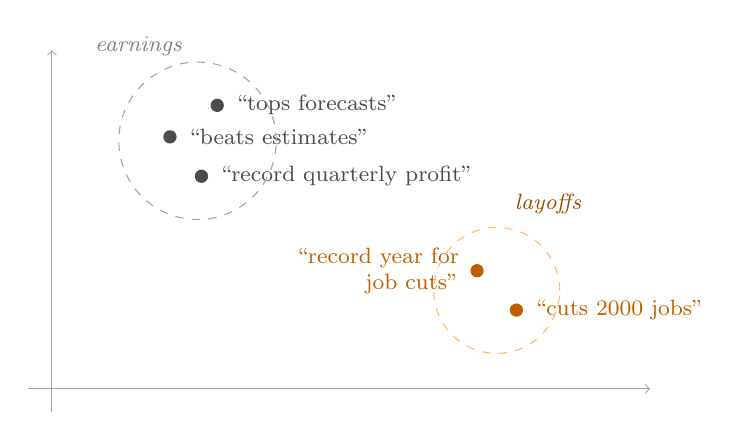
\begin{tikzpicture}[font=\small]
  \draw[->, black!35] (-0.3,0) -- (7.6,0);
  \draw[->, black!35] (0,-0.3) -- (0,4.3);
  % cluster resultados
  \fill[black!70] (1.5,3.2) circle (2.4pt) node[right=3pt, align=left, font=\footnotesize] {``beats estimates''};
  \fill[black!70] (2.1,3.6) circle (2.4pt) node[right=3pt, align=left, font=\footnotesize] {``tops forecasts''};
  \fill[black!70] (1.9,2.7) circle (2.4pt) node[right=3pt, align=left, font=\footnotesize] {``record quarterly profit''};
  \draw[black!35, dashed] (1.85,3.15) circle (1.0);
  \node[black!50, font=\footnotesize\itshape] at (1.1,4.35) {earnings};
  % cluster despedimentos
  \fill[orange!75!black] (5.9,1.0) circle (2.4pt) node[right=3pt, align=left, font=\footnotesize] {``cuts 2000 jobs''};
  \fill[orange!75!black] (5.4,1.5) circle (2.4pt) node[left=3pt, align=right, font=\footnotesize] {``record year for\\ job cuts''};
  \draw[orange!55, dashed] (5.65,1.25) circle (0.8);
  \node[orange!60!black, font=\footnotesize\itshape] at (6.3,2.35) {layoffs};
\end{tikzpicture}
\caption[Sentences as points in a space]{Each sentence corresponds to a point in the space.
Sentences of close meaning occupy neighbouring positions even when they share no vocabulary,
whereas sentences with common vocabulary (``record'') and distinct subject end up far apart. The
representation is two-dimensional to allow it to be read; the model uses 384 dimensions.}
\label{fig:met_embeddings}
\end{figure}

The measurement of the outcome adapts the event study \autocite{brown1985daily}: with the day of
the news fixed, the price change is measured at one, three and five days. Two detailed decisions
condition the result. News published outside trading days is aligned with the first following
trading day. The measurement begins at the close of the day of the news, and not at the open, a
conservative option that avoids attributing to the news the part of the movement prior to its
publication.

The value presented to the user is the raw return and not the abnormal return the source
normalises. The option is deliberate and has a declared cost. The raw return is verifiable by the
user in their own application, but it incorporates the movement of the market over the period. In
periods of generalised decline, the precedents appear to have worse outcomes than those
attributable to the news. The market is discounted where it is indispensable, in the construction
of the label described in the following section.


\section{News triage}
\label{sec:met_triagem}

The fourth decision determines which news items justify interrupting the user. Unlike the previous
ones, it has no obvious analytical formulation, and constitutes the natural point for learning from
the data.

The label formalises the question as the occurrence of an abnormally large movement after the
news. The return of the stock over the following three days is measured, the movement of the market
over the same period is subtracted, and the example is classified as positive when the absolute
value of the residual exceeds two per cent. The use of the absolute value is deliberate: the model
learns about materiality and never about direction, which preserves the founding constraint of the
work.

Subtracting the movement of the market assumes unit sensitivity, which is an inconsistency with
the technique described in Section~\ref{sec:met_decomposicao}, which refuses precisely that
assumption. In a high-beta stock, the residual retains part of the movement of the market, and the
label may classify as material a day on which only the market moved. All the families of model
evaluated in Chapter~\ref{cap:avaliacao} are trained and evaluated against the same label, so the
comparison between them is internally consistent under this definition of target. That does not
guarantee, however, that the ordering survives an alternative definition, since the error
introduced may be correlated with the company and with volatility.

The model receives nine inputs: the volatility of the twenty preceding days, the momentum of the
five preceding days, the return of the day itself, the length of the headline and five sector
indicators. An additional variant incorporates the 384-dimensional vector of the headline.
Figure~\ref{fig:met_entradas} groups the inputs by the level of information each one describes, a
distinction that Chapter~\ref{cap:avaliacao} shows to be decisive.

\begin{figure}[ht]
\centering
\begin{tikzpicture}[font=\footnotesize, >={Stealth[length=2mm]},
  cx/.style={draw, rounded corners=2pt, align=center, inner sep=3pt, minimum height=0.62cm,
             text width=2.35cm},
  emp/.style={cx, fill=black!8},
  dia/.style={cx, fill=black!16},
  not/.style={cx, fill=black!45, text=white, draw=black!60, very thick},
  rot/.style={font=\scriptsize\bfseries, text=black!65, align=left},
]
  % nivel EMPRESA: sete entradas
  \node[rot] at (-2.55,0.62) {COMPANY level};
  \node[emp] (a) at (0,0)    {20-day\\ volatility};
  \node[emp] (b) at (2.6,0)  {5-day\\ momentum};
  \node[emp] (c) at (5.2,0)  {sector: banking};
  \node[emp] (d) at (7.8,0)  {sector: consumer};
  \node[emp] (e) at (0,-0.95)   {sector: energy};
  \node[emp] (f) at (2.6,-0.95) {sector: health};
  \node[emp] (g) at (5.2,-0.95) {sector: technology};
  \node[font=\scriptsize, text=black!55, align=left, text width=2.4cm]
    at (7.9,-0.95) {change slowly, or not at all};

  % nivel DIA
  \node[rot] at (-2.55,-1.95) {DAY level};
  \node[dia] (h) at (0,-2.15) {same-day\\ return};
  \node[font=\scriptsize, text=black!55, align=left, text width=5.6cm]
    at (4.3,-2.15) {identical for every headline of the same company that day};

  % nivel NOTICIA
  \node[rot] at (-2.55,-3.15) {HEADLINE level};
  \node[not] (i) at (0,-3.35) {headline\\ length};
  \node[font=\scriptsize, text=black!70, align=left, text width=5.6cm]
    at (4.3,-3.35) {\textbf{the only one that separates two headlines of the same company on the same day}};

  \draw[black!25] (-3.9,-1.55) -- (9.3,-1.55);
  \draw[black!25] (-3.9,-2.75) -- (9.3,-2.75);
\end{tikzpicture}
\caption[The nine inputs, by level]{The nine inputs of the deployed model, grouped according to
what each one allows to be distinguished. Seven characterise the \textbf{company} and vary slowly
or stay constant; one characterises the \textbf{day} and takes the same value for every news item
of that day; \textbf{only one} varies between consecutive headlines. From this composition follows
the expectation that the model does not separate two news items of the same company on the same
day, an expectation the ablation of Section~\ref{sec:av_ablacao} confirms.}
\label{fig:met_entradas}
\end{figure}

Seven inputs describe the company and vary slowly or are constant; one describes the day and is
identical for every news item of that day; and only one, the length of the headline, distinguishes
two headlines of the same company on the same day.

The split of the data is chronological and not random, as shown in
Figure~\ref{fig:met_divisao}. A random split would allow training on news posterior to that used in
the evaluation, inverting the temporal order the system faces in operation. Between consecutive
blocks there is a five-day embargo, necessary because the label of a news item depends on the
following three days: without the embargo, the label of the news items at the end of a block would
be determined by days belonging to the following block. The embargo discards 820 of the 79{,}753
rows, that is, $1.03\%$, leaving 28{,}574 examples for training, 17{,}710 for validation and
32{,}649 for testing.

\begin{figure}[ht]
\centering
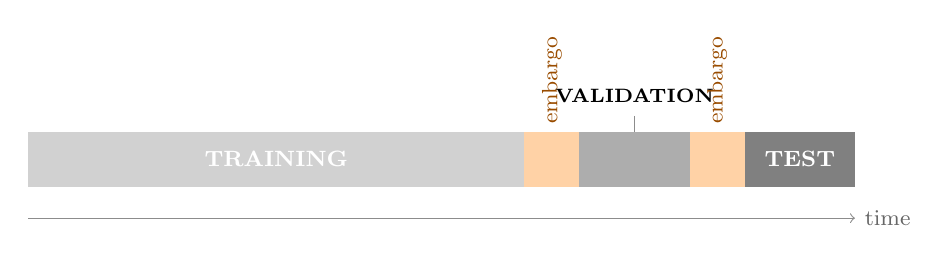
\begin{tikzpicture}[font=\small]
  \fill[black!18] (0,0) rectangle (6.3,0.7);
  \fill[orange!35] (6.3,0) rectangle (7.0,0.7);
  \fill[black!32] (7.0,0) rectangle (8.4,0.7);
  \fill[orange!35] (8.4,0) rectangle (9.1,0.7);
  \fill[black!50] (9.1,0) rectangle (10.5,0.7);
  \node[white, font=\footnotesize\bfseries] at (3.15,0.35) {TRAINING};
  % ⚠️ "VALIDAÇÃO" é mais larga do que o seu bloco (1.4 cm) e derramava sobre as duas bandas
  % do embargo, de um lado e do outro. Sai para cima, com um traço a apontar-lhe. Alargar o
  % bloco não servia: as larguras são as proporções reais do eixo do tempo.
  \node[font=\scriptsize\bfseries, anchor=south] (rotval) at (7.7,0.95) {VALIDATION};
  \draw[black!45] (7.7,0.9) -- (7.7,0.7);
  \node[white, font=\footnotesize\bfseries] at (9.8,0.35) {TEST};
  \node[orange!60!black, font=\footnotesize, rotate=90] at (6.65,1.35) {embargo};
  \node[orange!60!black, font=\footnotesize, rotate=90] at (8.75,1.35) {embargo};
  \draw[->, black!45] (0,-0.4) -- (10.5,-0.4) node[right, black!60, font=\footnotesize] {time};
\end{tikzpicture}
\caption[Temporal split with embargo]{The split of the data follows \textbf{chronological order}
and not a draw. Between consecutive blocks a five-day \emph{embargo} is inserted, since the label
of each news item depends on the following three days: without it, the end of the training block
would be determined by days belonging to the following block.}
\label{fig:met_divisao}
\end{figure}

The chronological discipline is a claim about what the dataset contains, and a claim of that
nature is not established by declaration. It is therefore enforced by an executable procedure,
reproduced in Listing~\ref{lst:lookahead}, which builds two series identical up to the day of the
news item and divergent after it, and requires the two properties that separate a legitimate input
from a leak: the inputs of the model have to remain equal, and the label has to change. An input
that came to depend on the future would break the first equality; a label that did not depend on
it would break the second.

\begin{lstlisting}[caption={[The test that mutates the future]The procedure that enforces the
temporal separation. The two series coincide up to the day of the event and diverge afterwards.
The inputs have to come out identical, because none of them may observe the future; the labels
have to come out different, because it is precisely the future that they measure. The test runs
on every execution of the automatic verification. Identifiers and comments are in the
original.}, label={lst:lookahead}]
def test_anti_lookahead_mutar_o_futuro_muda_o_rotulo_mas_nao_as_features():
    base = [100.0] * 25
    sobe = _serie(base + [100, 110, 120, 130])   # movimento anormal enorme
    plano = _serie(base + [100, 100, 100, 100])  # nada acontece
    mercado = _serie([100.0] * 29)
    d = 25
    assert event_features(sobe, d) == event_features(plano, d)          # features iguais
    assert abnormal_label(sobe, mercado, d, 0.02, 3) == 1               # rótulos diferentes
    assert abnormal_label(plano, mercado, d, 0.02, 3) == 0
\end{lstlisting}

The test block contains more examples than the training block. The cut is made on trading days,
according to a proportion of seventy, fifteen and fifteen per cent, and the asymmetry results from
the density of news, which grows markedly over the period covered by the corpus. Splitting by days,
and not by number of examples, is necessary so that news items of the same day are not distributed
across distinct blocks.

The score produced by the model is not, in itself, a probability. Since the value is presented to
the user, it is converted through \emph{post-hoc} calibration, fitting a two-parameter sigmoid over
the held-out validation block \autocite{niculescu2005calibration}:

\begin{equation}
p_{\text{calibrated}} = \frac{1}{1 + e^{-(a\,p_{\text{raw}} + b)}}
\label{eq:platt}
\end{equation}

The learned values are $a = 3.700$ and $b = -2.313$. The negative sign of $b$ indicates that the
model, without calibration, produces values systematically above the observed frequency. Part of
this behaviour follows from the reweighting of the classes during training, which shifts the scores
upwards by construction.

The calibration is fitted on a block whose prevalence of positive cases differs from that of the
test block, a consequence of the chronological split. The effect is measurable and is reported in
Chapter~\ref{cap:avaliacao}. The transformation is monotonic and preserves the ordering between
news items, which is what the decision policy uses; it is the absolute value presented that is
affected.

\section{Tools and infrastructure}
\label{sec:met_ferramentas}

The system is written in Python 3.12. The dependencies that produce the results of this
dissertation are pinned to exact versions, and not to ranges, so that the environment can be
recreated on another machine: \texttt{numpy}~2.1.3, \texttt{pandas}~2.2.3,
\texttt{scikit-learn}~1.9.0, \texttt{matplotlib}~3.11.0, \texttt{sentence-transformers}~5.6.0 and
\texttt{torch}~2.12.1 in the CPU variant. No result requires a graphics processing unit, a
consequence of the options described in this chapter.

All data sources are free. Prices come from a chain of alternative providers consulted in a fixed
order, since no free source is sufficiently reliable on its own; the system always records which
one answered. News comes from three complementary providers, whose comparison is presented in
Chapter~\ref{cap:sistema}. Delivery uses the Telegram bot interface.

\section{Technological and social challenges}
\label{sec:met_desafios}

This section states the risks that a system with these characteristics raises and the design
decisions that respond to each of them.

\subsection{Privacy and data protection}
\label{sec:met_privacidade}

An investment portfolio reveals income, risk aversion and life plans, information that the General
Data Protection Regulation treats as deserving reinforced protection when it allows a person to be
profiled.

The design decision that responds to this risk is minimisation: the system does not know the
users' positions and does not ask for them. There is no portfolio, there are no positions and no
amounts, and the public channel does not identify recipients. An alert about a company is identical
for every reader. The cost of this option is the impossibility of personalisation, since the system
alerts on a fixed list of companies and not on the positions of whoever reads it.

There is one exception worth naming. Users who choose to receive personalised alerts through the
Telegram bot are associated with two elements: the conversation identifier assigned by the platform
and the list of companies selected. No name, contact or amounts are stored. The processing rests on
the express request of the user, who begins it by subscribing and ends it through a command that
deletes the record.

\subsection{Security}
\label{sec:met_seguranca}

An autonomous system that consumes external services holds credentials. The keys reside in
environment variables and in the platform's secret store, never in the repository, and the text
sent to the logs passes through a function that masks parameters with a credential name. This
second safeguard responds to the fact that the error messages of communication libraries reproduce
the address of the request, and that some interfaces carry the key in that address.

The sentence encoder is fetched on demand and checked against a checksum fixed in the code.
Without that verification, a corrupted or substituted file would silently modify the similarity
criterion used by the system.

\subsection{Ethical and social questions}
\label{sec:met_etica}

The founding constraint of the work is also its main ethical safeguard. A system that announced
the future behaviour of the price would issue a forecast not verifiable at the moment of reading; a
system that indicated instruments to buy would enter a regulated activity. This boundary is one of
design, drawn out of prudence and not from an analysis of the applicable law: there was no legal
opinion, and operating the system as a service would require obtaining one first.

The guarantee applies to what the system writes and not to what it reproduces. Third-party
headlines are quoted in full, since they constitute the fact that triggers the alert and allow
verification at the source, and some are themselves speculative. From this follows a limitation
without a solution within the scope assumed: the relevance filter determines whether a headline is
about the company, and not whether it is factual. The distinction between news and opinion would
require a classifier the system does not have.

Repeated interruption is the second risk. The effect is documented in clinical decision support
systems, where \textcite{ancker2017alertfatigue} measure that the probability of accepting an alert
decreases as the volume of alerts received increases, and that the effect is accentuated by
repetition of the same alert. The domain is distinct and what transfers is the mechanism: whoever
is interrupted frequently stops distinguishing the interruptions, from which point a correct
warning and an incorrect warning have the same effect. The system responds with a daily alert
budget, a rising threshold for repeated alerts of the same company, and suppression of news that
reproduces a story already communicated.

The third risk follows from the explanation itself. Trust in automated systems fails in both
directions, with the user ignoring a correct warning or accepting an incorrect one
\autocite{lee2004trust}, and the presence of an explanation increases the acceptance of wrong
answers \autocite{bansal2021whole}. The system therefore presents past cases individually, with
date and outcome, rather than summarising them into an average liable to be read as a forecast.
That this option produces appropriate trust is a hypothesis and not a result, since the controlled
study needed to verify it was not carried out.


\subsection{Use of artificial intelligence tools}
\label{sec:met_ia}

This subsection declares, as the Statement of Integrity refers, how generative artificial
intelligence tools were used in this work and for what purpose.

The conception is the author's: the problem, the research questions, the constraints that define
the system (free sources only, explainability first, and the refusal to forecast prices), the
design of each experiment, the success criterion fixed before running it, and every decision about
what to build, keep or discard. No conclusion in this document was delegated.

The execution was assisted, and to a substantial extent. Those tools wrote and restructured a
considerable part of the system's code and of its tests, implemented the evaluation procedures,
drafted and edited prose in this document, and conducted reviews that found defects in the software
and in the text. Where a measurement contradicted a claim of the author, the claim was withdrawn
rather than defended, and Appendix~\ref{ap:reprodutibilidade} records those that were withdrawn.

The content of this document was reviewed by the author. It, the errors that remain in it, and
its defence are his responsibility.